In der Landwirtschaft geht es häufig darum, Sachen (Flüssigkeiten,Samen,etc.)
auf dem Feld auszubringen. Auf die herkömmliche Art macht das ein Bauer,
mithilfe eines Traktors. Je nach Aufgabe und Feldgröße benötigt ein Landwirt
hierfür mehrere kostbare Stunden. Die Ausbringung von Flüssigkeiten wäre ein
typischer Anwendungsfall für eine Drohne.

\begin{figure}[ht]
	\centering
	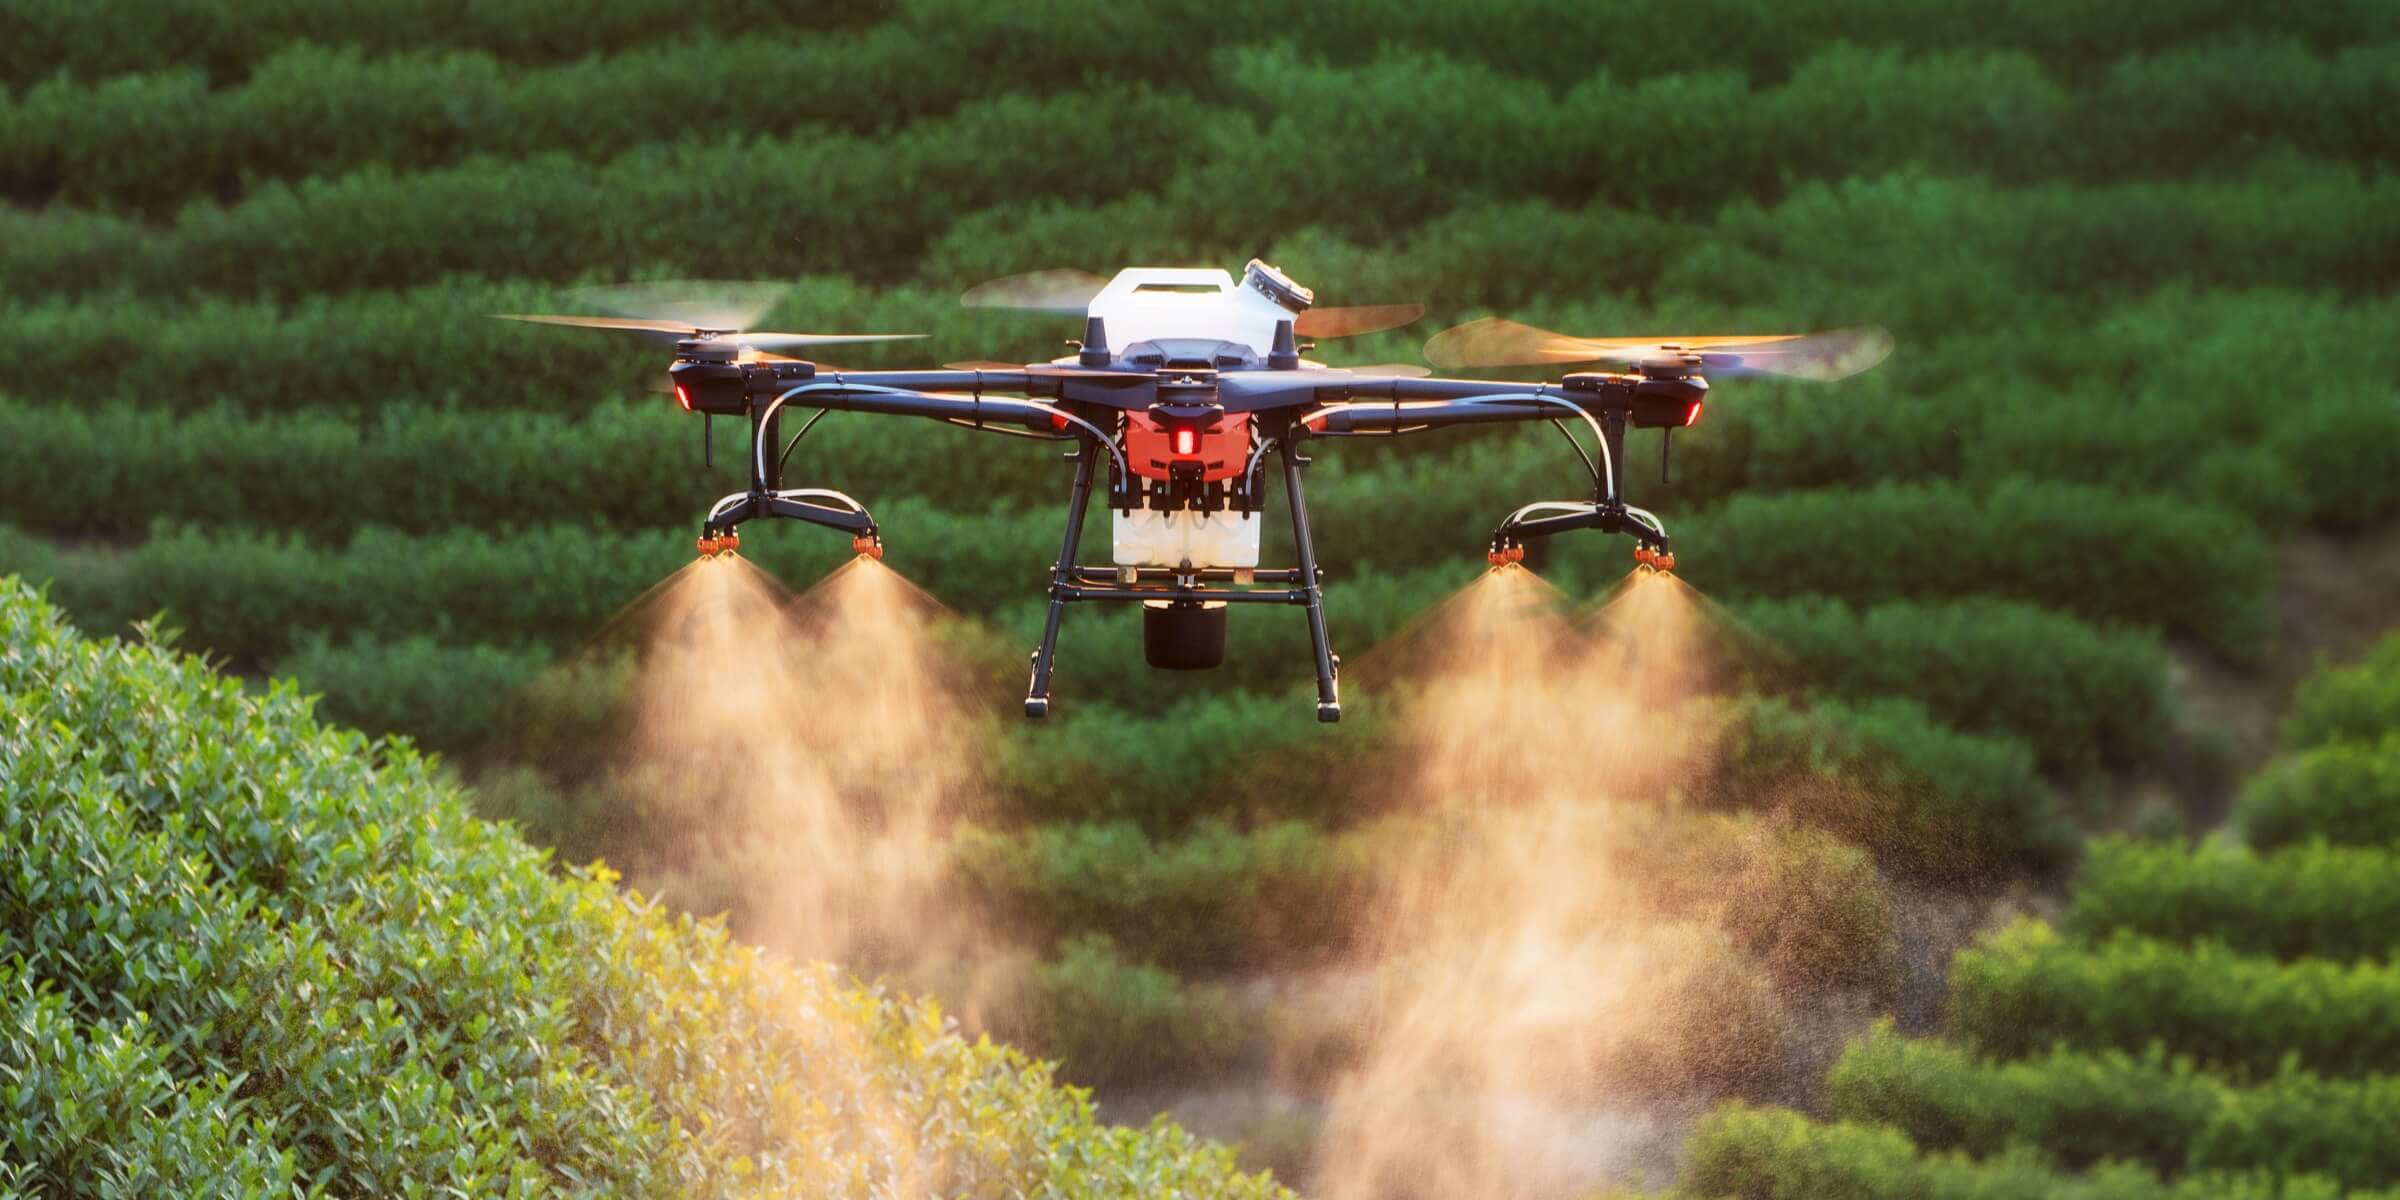
\includegraphics[width=0.7\textwidth]{bilder/drtohne.jpg}
	\caption[Sprühdrohne]{Sprühdrohne beim Aufbringen von Pestiziden \cite{Drohne}}
	\label{fig:sprühdrohne}
\end{figure}

Die Drohne in Abbildung \ref{fig:sprühdrohne} kann hierbei aus geringer Höhe
die entsprechenden Flüssigkeiten über eine Düse ausbringen. Das kann durch
Routenplanung komplett automatisiert passieren. Lediglich ein Flüssigkeitstank
ist hier benötigt, welcher jedoch innerhalb weniger Minuten vom Landwirt an
einer fest vorgegebenen Stelle platziert werden kann. Somit hat die Drohne
einen festen Bezugspunkt für das Auffüllen der Flüssigkeit, ähnlich einer
Ladestation eines Rasenmähers. \\ Ein zusätzliches weit verbreitetes
Einsatzgebiet von Drohnen im Allgemeinen ist die Überwachung: \\Auf den Feldern
wird dies häufig in Kombination mit Wärmebildkameras dazu verwendet, Tiere in
den Feldern aufzuspüren. Durch die Möglichkeit,
das Feld aus großen Höhen zu beobachten ermöglicht es dem Farmer, Rehe,
Wildschweine und andere Schädlinge schnell und effektiv in seinem Feld
aufzuspüren.
